
\documentclass[norsk,a4paper,12pt]{article}
\usepackage[T1]{fontenc} %for å bruke æøå
\usepackage[utf8]{inputenc}
\usepackage{graphicx} %for å inkludere grafikk
\usepackage{verbatim} %for å inkludere filer med tegn LaTeX ikke liker
\usepackage{mathpazo}
\usepackage{listings}
\bibliographystyle{plain}
\usepackage{xcolor}
\usepackage{float}
\usepackage{amsmath}

\definecolor{background}{gray}{0.95}
\definecolor{comment}{rgb}{0,0.5,0}
\colorlet{keyword}{blue}
\colorlet{string}{red}
\lstset{numbers=left,
	title=\lstname,
	numberstyle=\tiny, 
	breaklines=true,
	tabsize=4,
	language=Python,
	morekeywords={with,super,as},,
	frame=single,
	basicstyle=\footnotesize\tt,
	commentstyle=\color{comment},
	keywordstyle=\color{keyword},
	stringstyle=\color{string},
	backgroundcolor=\color{background},
	showstringspaces=false,
	numbers=left,
	numbersep=5pt,
	literate=
		{æ}{{\ae}}1
		{å}{{\aa}}1
		{ø}{{\o}}1
		{Æ}{{\AE}}1
		{Å}{{\AA}}1
		{Ø}{{\O}}1
	}



\title{Prosjekt}
\author{KANDIDATNUMMER}
\date{\today}
\begin{document}

\maketitle


\section*{Oppgave 1}
[ta med faseroms plott.]
\\
\\
Kan man bruke forskjellige initialbetingelser for å generere en bane som ikke er eliptisk, bruk totalenergien for å begrunne.
\\
\\
Hvorfor står banen i faserommet vinkelrett på x og y aksen?
\\
\\
Beverger plotet seg med eller mot klokka? Plott litt mindre enn en runde og se. Kan den gå motsatt retning?
\\
\\


Se plot for plot, kode for kode.
\\
\\
\begin{figure}[H]
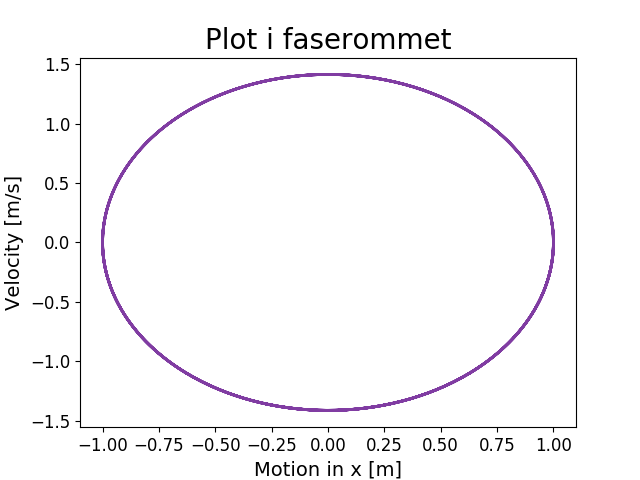
\includegraphics[scale=0.8]{Oppgave1.png}
\end{figure}


Energien for en fjerpendel
\\
\\
Totalenergien viser et eller annet, FINN UT AV HVA TOTALENERGIEN ER. Siden det ikke er noen form for friksjon så vil energien bare veksle mellom potensiell og kinetisk. + mer forklaring
\\
\\
\\
\\
\\
\\
Systemet i faserommet beveger sem med klokka. Det går ikke ann å bruke en kombinasjon av initialverdier til å få den til å gå motsatt retning, fordi det avhenger av hvordan vi har satt positiv retning.  SIKKERT IKKE HELT RIKTIG ELLER KOMPLETT, SÅ DISKUTER LITT OG SKRIV BEDRE




\section*{Oppgave 2}
Diskuter banen i faserommet.
\\
\\
Står banen fortsatt loddrett på begge aksene. Nei, men står den vinkelrett, det kan du finne ut av.
\\
\\
Hva er en attraktor?
\\
\\
En attraktor er et set med numeriske verdier som et dynamisk system har en tendens til å utvikle seg mot for et bredt utvalg av initialbetingelser. En attraktor kan være et punkt(1 dim), et set met punkter(Jeg syntes 1 dim også), en kurve(2 dim), og flere ting innenfor matematikk. Punktet $x=0m$ og $\dot{x}=0m/s$ er en attraktor av dimensjon 1, fordi det er et singulært punkt. Kurven i oppgave 1 er også en attraktor i følge definisjonen tror jeg, siden systemet alltid havner i den kurven uansett initialbetingelser. På den andre siden så kan det argumenteres for at det ikke er en attraktor fordi systemet faktisk ikke kan gjøre noe annet, og dermed ikke kan ha en tendens til å ende langs kurven. Altså siden den ikke begynner utenfor kurven og så går inn og blir der så er det ikke en attraktor. FINN UT AV DET.



\begin{figure}[H]
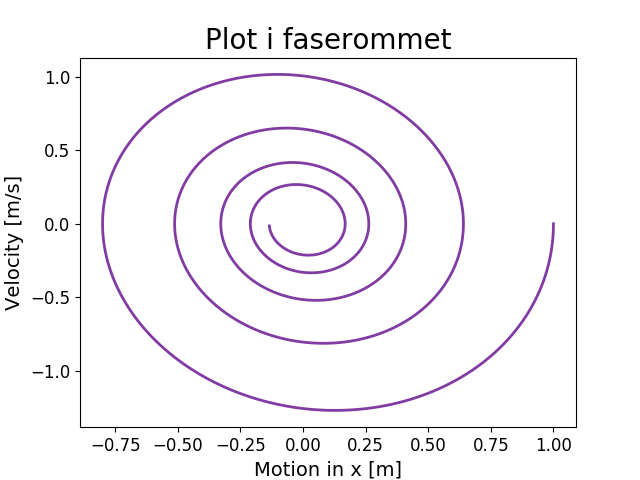
\includegraphics[scale=0.8]{Oppgave2.png}
\end{figure}


\section*{Oppgave 3}

Vi skal løse følgende likning alanytisk.
\\
\\
\begin{equation}
	m \ddot{x}(t) +kx(t) = F_D cos(\omega_Dt)
\end{equation}

Begynner med å finne den generelle løsningen for den homogene likningen, og løser derfor den karakteristiske likningen $m\lambda^2 + k = 0$

\begin{align*}
	m\lambda^2 + k =& 0 \\
	\lambda^2 =& \frac{-k}{m} \\
	\lambda =& \pm \sqrt{\frac{-k}{m}}\\
\end{align*}

Hvis vi har $\lambda$ på formen $\lambda_{\pm} = \mu \pm i\eta$, så får vi den generelle løsningen

\begin{align*}
	\lambda =& \pm i \sqrt{\frac{k}{m}}\\
	x_h =& e^{\mu t}(A cos(\eta t) + B sin(\eta t))\\
	x_h =& e^{0t}(A cos(\sqrt{\frac{k}{m}}t) +B sin(\sqrt{\frac{k}{m}}t))\\
	x_h =& \underline{A cos(\sqrt{\frac{k}{m}}t) +B sin(\sqrt{\frac{k}{m}}t)}\\
\end{align*}

Så den generelle løsningen for den homogene delen er

\begin{equation}
	x_h = A cos(\sqrt{\frac{k}{m}}t) +B sin(\sqrt{\frac{k}{m}}t)
\end{equation}


Nå skal vi bruke metoden for ubestemte koeffisienter for å finne den partikulære løsningen. Siden høyre side av likningen er på formen $A cos(pt)$, så kan vi bruke $x_p$ på formen $C e^{ipt}$

\begin{align*}
	x_p =& C e^{ipt},\   \   \ p=\omega_D, fra\ \ likningen
\end{align*}

Hvordan kan vi tolke en slik løsning?
\\
\\

\section*{Oppgave 4}

Det nummeriske resultatet bør være det samme som det analytiske. Er bevegelsen periodisk?
\\
\\
Med ny $\omega_D$ er bevegelsen fortsatt periodisk. Begrunn svaret. Finn definisjon av periodisk bevegelse.

\begin{figure}[H]
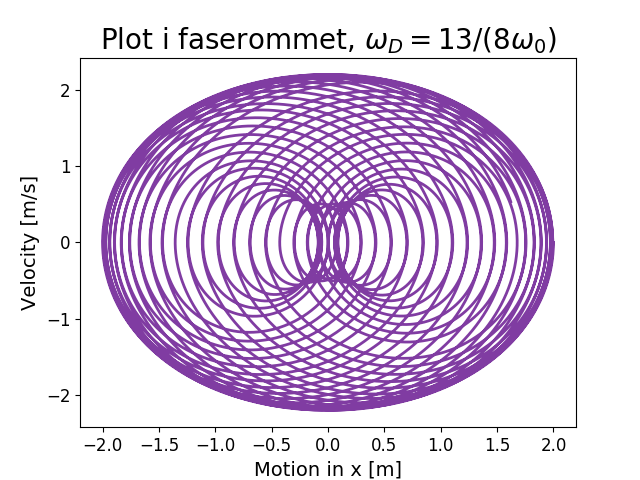
\includegraphics[scale=0.8]{Oppgave4del1.png}
\end{figure}

ting
Lorem ipsum dolor sit amet, consectetur adipiscing elit. Nulla sed massa urna. Fusce placerat, nulla id aliquam varius, nulla risus commodo metus, in fringilla velit massa eu odio. Aliquam vitae eros at orci volutpat pulvinar eu a sapien. Proin ullamcorper tincidunt orci vel vehicula. Vestibulum venenatis eget magna at pharetra. Aenean ut rutrum urna. Aliquam venenatis leo viverra, fermentum massa vel, maximus lectus. Pellentesque pulvinar sodales massa non venenatis. Praesent lobortis consequat erat ut semper. Nulla tincidunt ac enim sed imperdiet. Nulla maximus dui eget eros laoreet, vitae eleifend magna vulputate. Sed ut molestie neque. Sed sagittis sagittis metus. Fusce placerat enim ut augue ornare mattis.
\\

\begin{figure}[H]
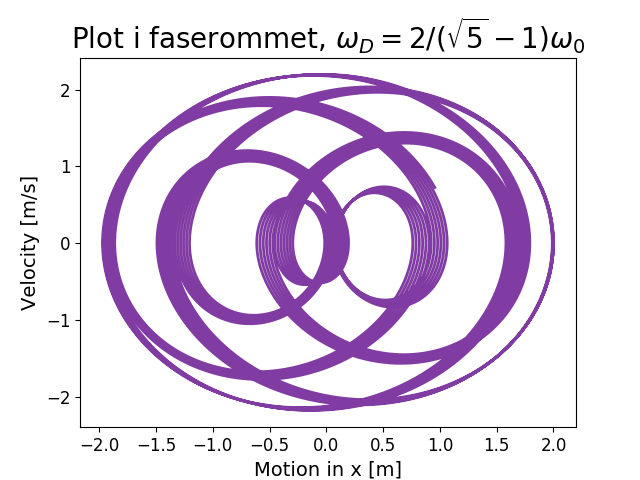
\includegraphics[scale=0.8]{Oppgave4del2.png}
\end{figure}


Lorem ipsum dolor sit amet, consectetur adipiscing elit. Nulla sed massa urna. Fusce placerat, nulla id aliquam varius, nulla risus commodo metus, in fringilla velit massa eu odio. Aliquam vitae eros at orci volutpat pulvinar eu a sapien. Proin ullamcorper tincidunt orci vel vehicula. Vestibulum venenatis eget magna at pharetra. Aenean ut rutrum urna. Aliquam venenatis leo viverra, fermentum massa vel, maximus lectus. Pellentesque pulvinar sodales massa non venenatis. Praesent lobortis consequat erat ut semper. Nulla tincidunt ac enim sed imperdiet. Nulla maximus dui eget eros laoreet, vitae eleifend magna vulputate. Sed ut molestie neque. Sed sagittis sagittis metus. Fusce placerat enim ut augue ornare mattis.
\\


\section*{Oppgave 5}

Lorem ipsum dolor sit amet, consectetur adipiscing elit. Nulla sed massa urna. Fusce placerat, nulla id aliquam varius, nulla risus commodo metus, in fringilla velit massa eu odio. Aliquam vitae eros at orci volutpat pulvinar eu a sapien. Proin ullamcorper tincidunt orci vel vehicula. Vestibulum venenatis eget magna at pharetra. Aenean ut rutrum urna. Aliquam venenatis leo viverra, fermentum massa vel, maximus lectus. Pellentesque pulvinar sodales massa non venenatis. Praesent lobortis consequat erat ut semper. Nulla tincidunt ac enim sed imperdiet. Nulla maximus dui eget eros laoreet, vitae eleifend magna vulputate. Sed ut molestie neque. Sed sagittis sagittis metus. Fusce placerat enim ut augue ornare mattis.
\\
\\
mer ting
\begin{figure}[H]
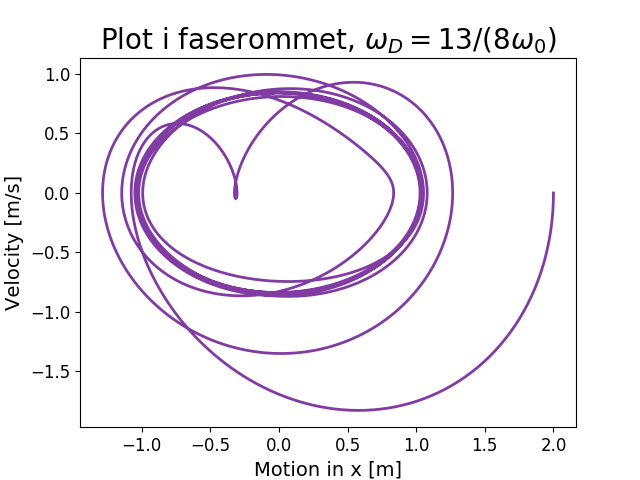
\includegraphics[scale=0.8]{Oppgave5del1.png}
\end{figure}


Lorem ipsum dolor sit amet, consectetur adipiscing elit. Nulla sed massa urna. Fusce placerat, nulla id aliquam varius, nulla risus commodo metus, in fringilla velit massa eu odio. Aliquam vitae eros at orci volutpat pulvinar eu a sapien. Proin ullamcorper tincidunt orci vel vehicula. Vestibulum venenatis eget magna at pharetra. Aenean ut rutrum urna. Aliquam venenatis leo viverra, fermentum massa vel, maximus lectus. Pellentesque pulvinar sodales massa non venenatis. Praesent lobortis consequat erat ut semper. Nulla tincidunt ac enim sed imperdiet. Nulla maximus dui eget eros laoreet, vitae eleifend magna vulputate. Sed ut molestie neque. Sed sagittis sagittis metus. Fusce placerat enim ut augue ornare mattis.
\\
ting


\begin{figure}[H]
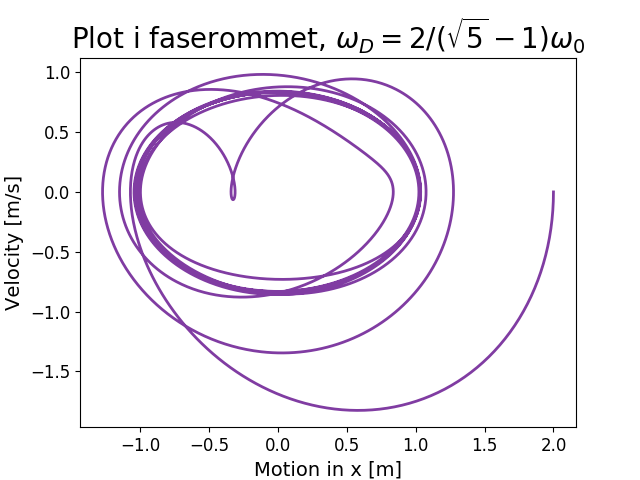
\includegraphics[scale=0.8]{Oppgave5del2.png}
\end{figure}

Lorem ipsum dolor sit amet, consectetur adipiscing elit. Nulla sed massa urna. Fusce placerat, nulla id aliquam varius, nulla risus commodo metus, in fringilla velit massa eu odio. Aliquam vitae eros at orci volutpat pulvinar eu a sapien. Proin ullamcorper tincidunt orci vel vehicula. Vestibulum venenatis eget magna at pharetra. Aenean ut rutrum urna. Aliquam venenatis leo viverra, fermentum massa vel, maximus lectus. Pellentesque pulvinar sodales massa non venenatis. Praesent lobortis consequat erat ut semper. Nulla tincidunt ac enim sed imperdiet. Nulla maximus dui eget eros laoreet, vitae eleifend magna vulputate. Sed ut molestie neque. Sed sagittis sagittis metus. Fusce placerat enim ut augue ornare mattis.
\\
\\

\section*{Oppgave 6}

Lorem ipsum dolor sit amet, consectetur adipiscing elit. Nulla sed massa urna. Fusce placerat, nulla id aliquam varius, nulla risus commodo metus, in fringilla velit massa eu odio. Aliquam vitae eros at orci volutpat pulvinar eu a sapien. Proin ullamcorper tincidunt orci vel vehicula. Vestibulum venenatis eget magna at pharetra. Aenean ut rutrum urna. Aliquam venenatis leo viverra, fermentum massa vel, maximus lectus. Pellentesque pulvinar sodales massa non venenatis. Praesent lobortis consequat erat ut semper. Nulla tincidunt ac enim sed imperdiet. Nulla maximus dui eget eros laoreet, vitae eleifend magna vulputate. Sed ut molestie neque. Sed sagittis sagittis metus. Fusce placerat enim ut augue ornare mattis.
\\
\\

\section*{Oppgave 7}

Lorem ipsum dolor sit amet, consectetur adipiscing elit. Nulla sed massa urna. Fusce placerat, nulla id aliquam varius, nulla risus commodo metus, in fringilla velit massa eu odio. Aliquam vitae eros at orci volutpat pulvinar eu a sapien. Proin ullamcorper tincidunt orci vel vehicula. Vestibulum venenatis eget magna at pharetra. Aenean ut rutrum urna. Aliquam venenatis leo viverra, fermentum massa vel, maximus lectus. Pellentesque pulvinar sodales massa non venenatis. Praesent lobortis consequat erat ut semper. Nulla tincidunt ac enim sed imperdiet. Nulla maximus dui eget eros laoreet, vitae eleifend magna vulputate. Sed ut molestie neque. Sed sagittis sagittis metus. Fusce placerat enim ut augue ornare mattis.
\\
\\

\section*{Oppgave 8}

Lorem ipsum dolor sit amet, consectetur adipiscing elit. Nulla sed massa urna. Fusce placerat, nulla id aliquam varius, nulla risus commodo metus, in fringilla velit massa eu odio. Aliquam vitae eros at orci volutpat pulvinar eu a sapien. Proin ullamcorper tincidunt orci vel vehicula. Vestibulum venenatis eget magna at pharetra. Aenean ut rutrum urna. Aliquam venenatis leo viverra, fermentum massa vel, maximus lectus. Pellentesque pulvinar sodales massa non venenatis. Praesent lobortis consequat erat ut semper. Nulla tincidunt ac enim sed imperdiet. Nulla maximus dui eget eros laoreet, vitae eleifend magna vulputate. Sed ut molestie neque. Sed sagittis sagittis metus. Fusce placerat enim ut augue ornare mattis.
\\
\\

\section*{Oppgave 9}

Lorem ipsum dolor sit amet, consectetur adipiscing elit. Nulla sed massa urna. Fusce placerat, nulla id aliquam varius, nulla risus commodo metus, in fringilla velit massa eu odio. Aliquam vitae eros at orci volutpat pulvinar eu a sapien. Proin ullamcorper tincidunt orci vel vehicula. Vestibulum venenatis eget magna at pharetra. Aenean ut rutrum urna. Aliquam venenatis leo viverra, fermentum massa vel, maximus lectus. Pellentesque pulvinar sodales massa non venenatis. Praesent lobortis consequat erat ut semper. Nulla tincidunt ac enim sed imperdiet. Nulla maximus dui eget eros laoreet, vitae eleifend magna vulputate. Sed ut molestie neque. Sed sagittis sagittis metus. Fusce placerat enim ut augue ornare mattis.
\\
\\


\section*{Appendix}

\lstinputlisting{RK4.py}

\lstinputlisting{oppgave1.py}

\lstinputlisting{oppgave2.py}

\lstinputlisting{oppgave4.py}

\lstinputlisting{oppgave5.py}

\lstinputlisting{oppgave6.py}

%\lstinputlisting{oppgave7.py}

%\lstinputlisting{oppgave8.py}


\end{document}